\documentclass[11pt]{article}
\usepackage[utf8]{inputenc}
\usepackage{mystyle} 
\usepackage{mycommands}
\usepackage{parskip}


\title{Python for Data Analysis \\ \scalebox{0.62}{Lecture Notes}}

%\date{\scalebox{0.75}{\semester}}
\date{}
\author{\scalebox{0.81}{\link{https://github.com/alexanderthclark}{\instructor}} \\
	{
\includegraphics[width = 0.51cm]{crown_dark.png}} \\
  	{\scalebox{0.73}{\centering\emph{Columbia University SPS}}} }
    
  
\begin{document}

\maketitle


% Add note to reader
\paragraph{To the reader:} These are my lecture notes for Python for Data Analysis, which I consider a work in progress. They're not written to replace class attendance, so you might not find them self-contained. These notes rely on three books,
\begin{itemize}
    \item \textit{\link{https://www.pearson.com/us/higher-education/program/Gaddis-Starting-Out-with-Python-Plus-My-Lab-Programming-with-Pearson-e-Text-Access-Card-Package-4th-Edition/PGM335157.html}{Starting out with Python}} by Tony Gaddis
    \item \textit{\link{https://www.oreilly.com/library/view/python-for-data/9781491957653/}{Python for Data Analysis}} by Wes McKinney
    \item \textit{\link{https://www.oreilly.com/library/view/python-data-science/9781491912126/}{Python Data Science Handbook}} by Jake VanderPlas.
\end{itemize}
There are many other fantastic books and resources for self-studying Python. I encourage you to find as many supplementary sources as you find helpful, but to return to these notes to help focus on what will be important for doing well on assignments and exams in this course.  

\tableofcontents

% Insert lecture notes
\part{Lecture 1}

    \section{Course Overview}

Welcome! Please check Canvas for important announcements, materials, and links throughout the semester.
You'll also find course materials on Google Drive. Send me a request for access if the folder is not already shared with you. 

\smallskip
The point of the class is to learn Python \emph{for} \underline{data analysis}. 
This is not a computer science class and we will avoid taking too 
many detours that do not add meaningfully to a data analyst's/scientist's skillset. That means we'll learn 
enough syntax to manipulate data, analyze data, comfortably use existing packages, and write code for simple enough tasks where
there might not be a suitable function we can pull of the shelf.

\smallskip
We'll also be using Python 3. Syntax for Python 2 is slightly different, so don't be surprised if you find some
discrepancies in syntax in old Stack Exchange posts and in other resources. 


\subsection{Faculty}


\begin{lstlisting}[language = Python]
instructor, instructor_email = "Alexander Clark", "ac4725@columbia.edu"
# associate, associate_email = 
\end{lstlisting}

We're available by appointment and we'll set office hours based on the week.



\subsection{Books \& My Programming Lab}

To start, we're working from \emph{Starting out with Python} by Tony Gaddis. We'll use the accompanying My Programming Lab (MPL) exercises.
I'll have more to say about MPL later. My tentative plan is that MPL will be graded only to the requirement that you try half of the exercises.

\subsection{Software}

I think it's important we aren't dogmatic about the IDE or software we use, but you must download Anaconda. Contact me or the associate if you have trouble with the installation.
We'll work with Jupyter and Spyder. I also recommend you download Sublime Text or another simple text editor with synatax highlighting.
I will also use Google Colaboratory until we formally introduce Jupyter later in the course. 


\section{Why Python?}

First, what is Python? It's a high-level, general-purpose programming language. 
It is more general-purpose than a language like R. 
With libraries like pandas and scikit-learn available, it is now popular for data analysis.

Python's advantages over R are its readability and its popularity.

See the \link{https://www.python.org/dev/peps/pep-0020/}{Zen of Python} for design guidelines and \link{https://www.python.org/dev/peps/pep-0008/}{Pep 8} for a coding style guide.

You'll see Python in more job listings. I use Python every day, and I use R only occasionally for its more advanced statistical packages.

\begin{center}
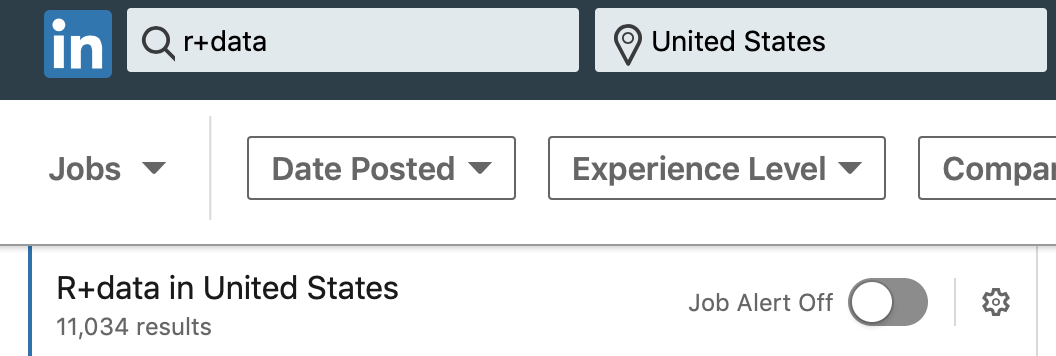
\includegraphics[width = .45\textwidth]{R_data_linkedin.png} 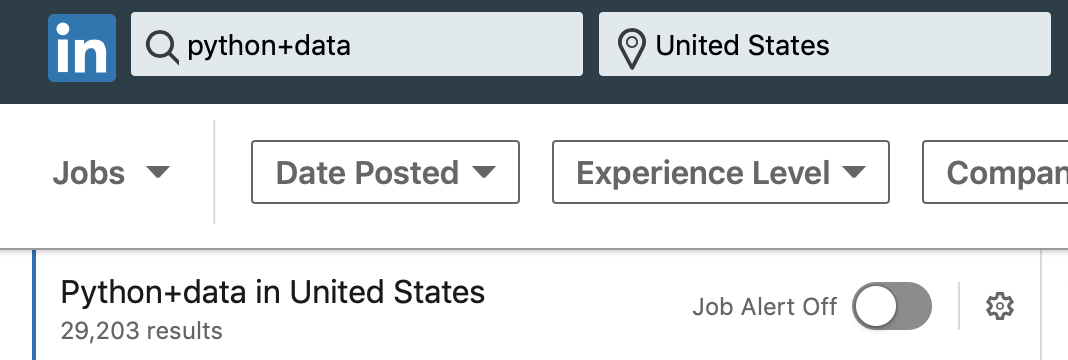
\includegraphics[width = .45\textwidth]{Python_data_linkedin.png}
\end{center}

\faMicrophone \faEyedropper.

\section{Input, Processing, and Output}
\scalebox{0.8}{\textit{Reference: Gaddis Chapter 2}}


\subsection{The Hello World Program (G\S 2.3)}

To get started in any langauge, printing ``Hello, World!'' might be the first step.\footnote{See
\textcolor{blue}{\href{https://en.wikipedia.org/wiki/\%22Hello,_World!\%22_program}
{the Wikipedia page for Hello, World.}}}

In Python, we can print an input using the \code{print()} function. We simply pass our
desired input within the parentheses, and Python will print the value.

We can enter text as a \textbf{string}. Text entered inside single, double, or triple quotations is interpreted as a string.


\begin{lstlisting}[language = Python]
print('Hello, World')
print("Hello, World!")
print("""Hello,
World!""") \end{lstlisting}


\smallskip
In Python 2, the syntax would have been \code{print 'Hello, World!'} without the parentheses.

\subsection{Comments (G\S 2.4)}

Commenting your code is helpful if you care about your colleagues or your future self. Comments should add clarity to
the intention and workings of code. A comment is a piece of code that isn't actually executed---it's a comment left for the reader or the person who inherits and modifies your code.
Everything after a \lstinline[language = Python]{#} will be ignored by the Python interpreter.

\begin{lstlisting}[language = Python]
# This will print a greeting.
print('Hello, World!') \end{lstlisting}

\smallskip
 You might also use end-line comments like the following

\begin{lstlisting}[language = Python]
print('Hello, World!') # Prints a greeting \end{lstlisting}

\smallskip

PEP 8 addresses comments \textcolor{blue}{\href{https://www.python.org/dev/peps/pep-0008/\#comments}{here}}.
I don't intend to grade based on the stylistic orthodoxy of your comments, but spaces are free so I do recommend 
\lstinline[language = Python]{# Comments like this} instead of \lstinline[language = Python]{#Comments like this}.


\subsection{Variables (G\S 2.5)}

A \textbf{variable} holds a value. It can be a string, a number, or perhaps a more complicated data type.
Variable assignment is done with the equals sign, \lstinline[language = Python]{=}.


\smallskip

\begin{lstlisting}[language = Python]
greeting = "Hello, World!"
my_favorite_number = 91 \end{lstlisting}

\smallskip

 Now compare the output you get from the following.

\begin{lstlisting}[language = Python]
print(greeting)
print('greeting')
print("Hello, World!")
print(91)
print(my_favorite_number)
print('my_favorite_number')
print("My favorite number is", my_favorite_number)
print("My favorite number is ", my_favorite_number) \end{lstlisting}


\smallskip

 PEP 8 addresses variable names \textcolor{blue}{\href{https://www.python.org/dev/peps/pep-0008/\#function-and-variable-names}{here}}.
Use lowercase and underscores.
This is good advice, but I don't see any reason to be too wedded to this. If you want to assign a matrix to a variable, 
it's reasonable to use an uppercase letter as the variable name. There, a math convention overrides a Python convention. Indeed, Gaddis is fine with uppercase (p. 43).

\smallskip

 More importantly, avoid Python key words in your variable names. \textcolor{blue}{\href{https://www.w3schools.com/python/python_ref_keywords.asp}
{Here}} is a list of keywords which have a specific meaning in code. An IDE will make this easier for you by highlighting keywords.

\begin{center}
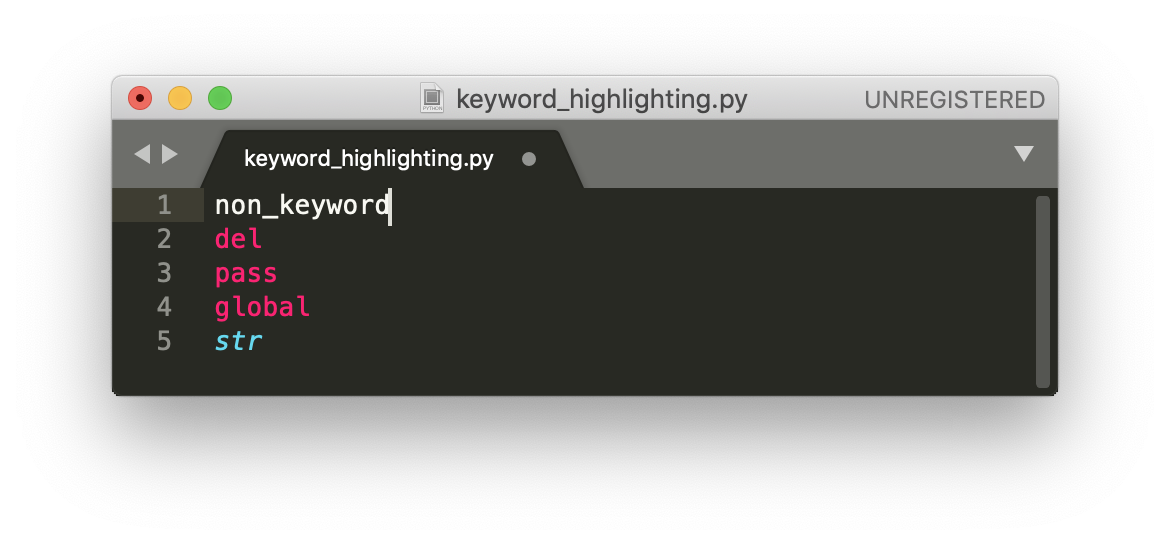
\includegraphics[width = .53\textwidth]{sublime_keyword_highlight.png}
\end{center}

\subsection{Data Types and Conversion (G\S 2.5, 2.6)}

To start, we are concerned with strings, integers, and floats. In Python, these are classes 
\lstinline{str}, \lstinline{int}, and \lstinline{float}.
You can check the type of variable or value using \lstinline[language = Python]{type()}.


\begin{lstlisting}[language = Python]
string_example = ''
int_example = -1
float_example = -1. \end{lstlisting}

\smallskip
 Some types can be converted by using \lstinline[language = Python]{str()},
\lstinline[language = Python]{int()}, or \lstinline[language = Python]{float()}.


\subsection{Input (G\S 2.6)}

It's not that common for a data science workflow, but you can read input using \lstinline[language = Python]{input()}.
The input is always read in as a string.

\begin{lstlisting}[language = Python]
favorte_color = input("What is your favorite color?")
favorite_number = input("What is your favorite number?")
attending_in_person = input("I am attending class in person.") \end{lstlisting}


\subsection{Calculations (G\S 2.7)}

You can use Python as a calculator. See the list of operations and symbols in Table 2-3 (Gaddis p. 54).
What might stand out is 
\begin{itemize}
\item Exponentiation is done with \lstinline[language = Python]{**}, not \lstinline[language = Python]{^}.
\item Integer division (rounds down) is done with \lstinline[language = Python]{//}.
\item The remainder of $x$ divided by $y$ can be found with \code{x \% y}, which might be read as
$x$ \emph{modulo} $y$. 
\end{itemize}

If a float is involved in an operation, the result will also be a float. 


\section{Decision Structures}
\scalebox{0.8}{\textit{Reference: Gaddis Chapter 3}}

Decision structures allow a program to have more than one path of execution. The path depends on condition. The condition is either True or False, and so can be represented by a Boolean variable.

\subsection{If Statements (G\S 3.1, 3.3)}

Here's a joke. A programmer is going to the grocery store and his partner says, ``Buy a gallon of milk, and if there are eggs, buy a dozen.''
The programmer comes home with 13 gallons of milk.

Or consider the logical inference if you ask, ``Is it raining?'' and get a reply, ``Not hard.'' 


\begin{lstlisting}[language = Python]
if 2 + 2 > 4:
    print("Pigs can fly.")
    
if 2 + 2 == 4:
    print("Pigs cannot fly.")
    
if 'a' < 'b':
    print("It is true that 'a' is less than 'b'.")
    
if 'a' < 'A':
    print("It is true that 'a' is less than 'A'.")
    
if 'goon' == 'Goblin':
    print("A goon is a goblin.") \end{lstlisting}
    
%https://genius.com/annotations/2257/standalone_embed

If statements like the above rely on \emph{relational operators} (see Table 3-1 Gaddis p.112).

\begin{lstlisting}[language = Python]
if 2 == 2.:
    print("The integer and the float are equal.")
    
if 2 is 2.:
    print("The integer and the float are the same object in memory.") \end{lstlisting}

\subsection{If Elif Else Statements (G\S 3.2, 3.4)}

Compare the output from the following programs.

\begin{lstlisting}[language = Python]
num = 0

if num < 1:
    print(num)
    num = num + 2
if num > 0:
    print(num, '!')
    num = num - 1000
if True:
    print(num, '?') \end{lstlisting}


\begin{lstlisting}[language = Python]
num = 0

if num < 1:
    print(num)
    num = num + 2
elif num > 0:
    print(num, '!')
    num = num - 1000
else:
    print(num, '?') \end{lstlisting}


\subsection{Logical Operators (G\S 3.5)}

Suppose you want to execute some code if a number $x$ is between 10 and 20. You could use \emph{nested} if statements.
\begin{lstlisting}[language = Python]
x = 14
if x >= 10:
    if x <= 20:
        print("x is between 10 and 20.") \end{lstlisting}
        

\smallskip
 But you might prefer to base your if statement off of one compound Boolean expression. For these, we need logical operations. They are

\begin{itemize}

\item Logical \textit{and}: \code{and} %, \lstinline[language = Python]{&}
\item Logical \textit{or}: \code{or} %, \lstinline[language = Python]{|}
\item Logical \textit{negation}: \code{not}
\end{itemize}
\smallskip

Observe the following will give equivalent output.

\begin{lstlisting}[language = Python]
not 1 > 2
not (1 > 2)
not(1 > 2) \end{lstlisting}


\smallskip

 \textbf{Challenge: } What do you expect from \lstinline[language = Python]{not not (1 or False)}?
        


\subsection{Boolean Variables (G\S 3.6)}

Finally, a Boolean variable simply references a logical True or False.

\begin{lstlisting}[language = Python]
# Option Value
market_value = 10
strike_price = 9
option_has_value = market_value > strike_price

if option_has_value:
    print("We're in the money.")
    
# Check data type
print(type(option_has_value)
print(type(False))) \end{lstlisting}

\part{Lecture 2}

    We now touch on lists (from Gaddis Chapter 7) and then go back to Chapters 4 and 5 to cover repetition structures and functions. 

\section{Lists}
\scalebox{0.8}{\textit{Reference: Gaddis Chapter 7}}

\subsection{Defining Lists (G\S 7.2)}

We have worked with strings, integers, floats, and booleans so far. Now, we introduce a compound data type the list.
Lists are also a sequence object, meaning they are ordered. 

A list is constructed by separating one or more objects with commas and placing them in square brackets. For example, we can define a list as follows.

\begin{lstlisting}[language = Python]
# Our first list---some Peloton content categories
floor = ['yoga', 'meditation', 'stretching', 'strength', 'cardiovascular'] \end{lstlisting}

\begin{lstlisting}[language = Python]
# More lists
aquatic = []
cycling = ['cycling'] \end{lstlisting}

\begin{lstlisting}[language = Python]
# More lists
treadmill_based = ['running', 'walking', 'bootcamp']  \end{lstlisting}

A useful quality of lists is that they can be of mixed type. 

\begin{lstlisting}[language = Python]
# More lists
fine_list = [0, 'milk', cycling]  \end{lstlisting}

\subsection{Indexing, Slicing, Mutating (G\S 7.2, 7.3)}

You can obtain the element at a certain place, or \emph{index}, in a list by suffixing the list with that index number inside square brackets. 
Python uses zero-based indexing. So one might say the $n^{\text{th}}$ item is at index $n-1$. This can create confusion when talking about the first, second, etc items in a list. I'll try always to speak of elements \emph{at index} zero, one, etc, so that you know I am referring to the position according to this zero-based system. 

\begin{lstlisting}[language = Python]
# Get specific items
fine_list = [0, 'milk', cycling]

# Which of these print statements will raise an error?
print(fine_list[0])
print(fine_list[1])
print(fine_list[2])
print(fine_list[3])
print(fine_list[-1])) \end{lstlisting}


We can also count from the end of the list to find an item, as hinted by the 
\code{fine_list[-1]} above. The index $-1$ will identify the last element. So, in some sense, you might say that negative indexing
is not zero-based though it is in fact consistent with the zero-based indexing described above. If that's confusing, recall $-0 = 0$ and so \code{fine_list[-0]} 
is actually the same as \code{fine_list[0]}.


The following graphic helps explain how lists (and strings) are indexed.

\begin{figure}[h!] 
\begin{center} 
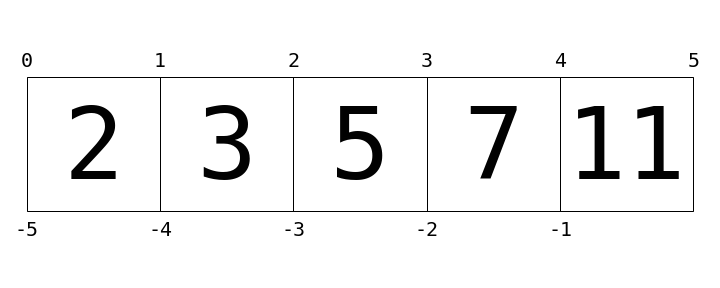
\includegraphics[width = .55\textwidth]{list_indexing.png}
\caption{Indexing (\textcolor{blue}{\href{https://jakevdp.github.io/WhirlwindTourOfPython/06-built-in-data-structures.html}{From \emph{Whirlwind Tour of Python} by Jake VanderPlas}}).}
\label{fig:while}
\end{center}
\end{figure}


%% Slicing

\bigskip

While indexing pulled out a single element, we can also \emph{slice} to pull out a sublist. 


\begin{lstlisting}[language = Python]
# Get specific items
['Jack', 'Jill', 'and', 'hill', 'over', 'ran', 'the']
print(fine_list[0:2])
print(fine_list[-2:]) \end{lstlisting}

The first print statement will print elements 0 and 1 in a list. The last print statement will print a list of just the last two elements.



%% Mutability 
\bigskip

Lists are \emph{mutable}, meaning that we can change their contents.


\begin{lstlisting}[language = Python]
# Get specific items
fine_list = [0, 'milk', cycling]
print(fine_list[0])
fine_list[0] = 1.0
print(fine_list[0]) \end{lstlisting}


\section{Repetition Structures}
\scalebox{0.8}{\textit{Reference: Gaddis Chapter 4}}

Repetition structures (loops) are one of the best justifications for moving from Excel to Python (though they are not unique to Python). A ``program''
in Excel is a serious of keystrokes and clicks. You might create a report for your company that is specific to one
market and you'll need to replicate the same report for a different market. Perhaps you could write a macro, but
I think you'll find working in Python to be easier. In Python, we can do this in a loop. We can have a program that makes the report and we
can iterate through the different markets to apply the program to each and create the specific reports (using a for loop).

\subsection{While Loops (G\S4.2)}
 
The \textbf{while loop} is a condition-controlled loop. Figure \ref{fig:while} illustrates the logic well. See also Figure 2 in Gaddis \S 4.2 (p. 163).

\begin{figure}[h!] 
\begin{center} 

\includegraphics[width = .55\textwidth]{while_loop.png}
\caption{While loop logic (\textcolor{blue}{\href{https://en.wikipedia.org/wiki/While\_loop}{Wikipedia}}).}
\label{fig:while}
\end{center}
\end{figure}


The statement inside a while loop executes as long as the condition evaluates to True.

\begin{lstlisting}[language = Python]
# Rest on the seventh day
day_of_week = 1
while day_of_week < 7:
    print('work')
    day_of_week += 1 \end{lstlisting}


Beware the infinite loop. Be confident that your test condition will have a way of becoming False, otherwise
you might notice that your program never finishes. 


Let's consider an infinite series, $\sum_{i=0}^\infty 2^{-i} =  1 + \frac{1}{2} + \frac{1}{4} + \frac{1}{8} + \dots = 2$.
We could try to calculate this with a while loop if we didn't know the sum converged to two.

\begin{lstlisting}[language = Python]
# Sum of a geometric series
the_sum = 0
idx = 0
increment = 2 ** -idx

while increment > 0:
    # Increase the sum by the current increment
    the_sum += increment
    
    # Advance the index in the sum and calculate a new increment
    idx += 1
    increment = 2 ** (-idx) \end{lstlisting}
    

Does this loop make you nervous? In fact, the loop will terminate because we will eventually hit machine zero.
I found the loop to terminate at the increment $2^{-1075}$ and the resulting sum to be two. But it should make you nervous.
You might instead decide on some level of precision and use a test condition like 
\code{increment > .0005}, in which case you could find a bound on the error with some math.
Doing that math is not part of this course, (un)fortunately.


\subsection{For Loops (G\S4.3)} 
\label{sec:forloop}

For loops execute the attached code based on some iteration. The code might depend on a variable that is actually changing
with the iteration. 

\begin{lstlisting}[language = Python]
# Dr. Seuss
for item in [1,2,'red','blue']:
    print(item, 'fish')  \end{lstlisting}


The for clause tells Python to execute the statement once for every item in the iterable, which is in this case the object \code{[1,2,'red','blue']}. This is a \emph{list}, a kind of 
compound data object that can store other objects in sequence by separating them with commas and putting them inside square brackets. Below we use \code{range(5)} instead of a list, which you can think of as generating an iterable object of integers from 0 to 4 (5 is not included, but the length is 5).


\smallskip

Or you might just want to execute a specific set of statements some number of times.


\begin{lstlisting}[language = Python]
# Tubthumping by Chumbawamba
for item in range(5):
    print("I get knocked down, but I get up again.")
    print("You are never gonna keep me down.") \end{lstlisting}

\smallskip

For both of the examples above, \code{item} is the \emph{variable}. However, notice
the print statement only depends on the variable in the first example.

\smallskip
You can even iterate over the characters in a string.

\begin{lstlisting}[language = Python]
# Cheer
word = 'PYTHON'
for char in word:
    print("Give me a",char, '!')
    print("    ", char)
print("What's that spell?")
print("    ",word) \end{lstlisting}


\subsection{Nested Loops (G\S 4.7)}

A loop that is inside another is called \emph{nested}.

\smallskip
Think about how Python executes code line by line. What order of output do you expect from this program?


\begin{lstlisting}[language = Python]
# Nested Loop
for x in ['wee', 'bee']:
    for y in ['bop', 'dop']:
        print(x,y) \end{lstlisting}


\smallskip




\section{Functions}
\scalebox{0.8}{\textit{Reference: Gaddis Chapter 5}}

\emph{Functions} make your code easier to read and reuse by performing a certain task based on some number of arguments
the function takes. 

In math, you might define a function $f(x) = x^2$. Just as $f$ does something with $x$, a function like 
\lstinline[language=Python]{print} does something with whatever input we pass inside the parentheses.

Consider the cheer we made in Section \ref{sec:forloop}. 

\begin{lstlisting}[language = Python]
# Cheer
word = 'PYTHON'
for char in word:
    print("Give me a",char, '!')
    print("    ", char)
print("What's that spell?")
print("    ",word) \end{lstlisting}


We can make this into a function. 


\begin{lstlisting}[language = Python]
# Cheer Function
def cheer(word):
    ''' Doc string '''
    for char in word:
        print("Give me a",char, '!')
        print("    ", char)
    print("What's that spell?")
    print("    ",word) \end{lstlisting}
    
Here's another function that takes a number and returns the next multiple of five by making use of a while loop. This is our first \emph{value-returning} function. Don't confuse the idea of a function returning something with simply doing something. The \code{cheer} function merely did something by printing a cheer. 

\begin{lstlisting}[language = Python]
# Find a nearby multiple of five
def find_close_multiple_of_five(num):
    # check if multiple of five
    is_multiple = num % 5 == 0
    while is_multiple not True:
        num += 1
        is_multiple = num % 5
    return num \end{lstlisting}
    
\section{Exercise}

\textbf{Hard}: Write a program that will find the first prime number after some given integer.

\vfill

\textit{Answers on next page.}

\pagebreak


\subsection{Exercise Answers}


\textbf{Hard}: Write a program that will find the first prime number after some given integer.

\begin{lstlisting}[language = Python]
# Find the first prime number greater than num.
# Initialize with a composite number
num = 20
is_prime = False

# Incremement the number until we find a prime.
while is_prime == False:
    num += 1
    is_prime = True # Initialize as prime and overwrite later
    
    for divisor in range(2,num): # Checks all integers >=2 and < num 
        if num % divisor == 0: # We enter the if statement when num/divisor is a whole number
            is_prime = False and is_prime # False along with and will make the whole boolean False
    # is_prime remains True when we exit the for loop not having found a single divisor \end{lstlisting}

\part{Lecture 3}

    \input{innards_03}

\part{Lecture 4}

    \input{innards_04}

\part{Lecture 5}

    \input{innards_05}

\part{Lecture 6}

    \input{innards_06}

\part{Lecture 7}

    \input{innards_07}

\part{Lecture 8}

    \input{innards_08}

\part{Lecture 9}

    \input{innards_09}

\part{Lecture 10}

    \input{innards_10}

\part{Lecture 11}

    \input{innards_11}

\end{document}
